% =========================================================
\section{Semaine 6 : Intégration Numérique}
% =========================================================

\textbf{But :} Calculer une approximation de $\int_a^b f(x)dx$, avec $f : [a, b] \to \mathbb{R}$ continue.

\subsection{Premières formules de quadrature}

\subsubsection*{Idée}

\begin{center}
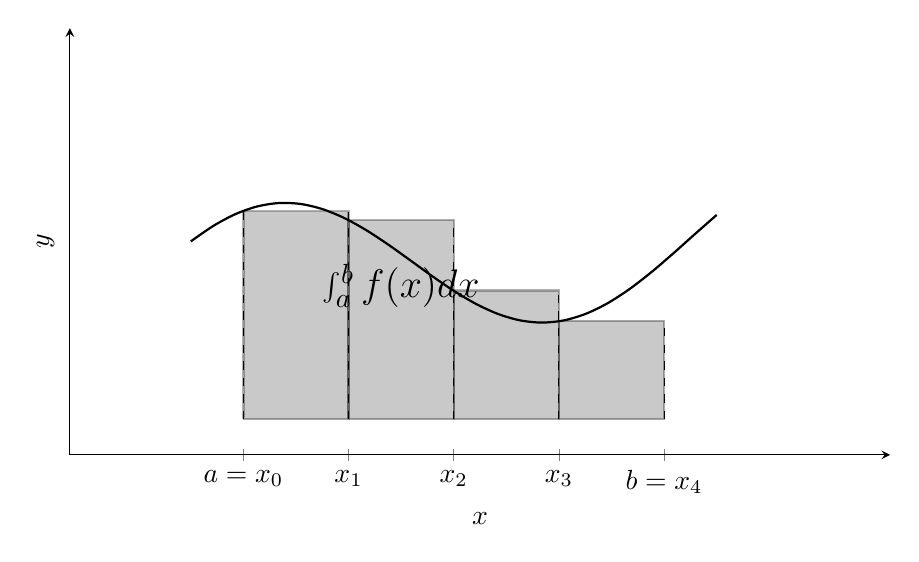
\begin{tikzpicture}
    \begin{axis}[
        axis x line=bottom,
        axis y line=left,
        ymin=0, ymax=4,
        xmin=0, xmax=6.5,
        xtick={1, 2, 3, 4, 5},
        xticklabels={$a=x_0$, $x_1$, $x_2$, $x_3$, $b=x_4$},
        ytick=\empty,
        xlabel={$x$},
        ylabel={$y$},
        width=12cm, height=7cm,
        enlargelimits=true,
        clip=false
    ]
    % Les rectangles pour la méthode du point gauche
    \addplot[fill=black!70, draw=black, thick, opacity=0.3] coordinates {(1,0) (1,2.34) (2,2.34) (2,0) (1,0)};
    \addplot[fill=black!70, draw=black, thick, opacity=0.3] coordinates {(2,0) (2,2.24) (3,2.24) (3,0) (2,0)};
    \addplot[fill=black!70, draw=black, thick, opacity=0.3] coordinates {(3,0) (3,1.45) (4,1.45) (4,0) (3,0)};
    \addplot[fill=black!70, draw=black, thick, opacity=0.3] coordinates {(4,0) (4,1.11) (5,1.11) (5,0) (4,0)};

    \draw[dashed] (1,0) -- (1,2.34);
    \draw[dashed] (2,0) -- (2,2.34);
    \draw[dashed] (2,0) -- (2,2.24);
    \draw[dashed] (3,0) -- (3,2.24);
    \draw[dashed] (3,0) -- (3,1.45);
    \draw[dashed] (4,0) -- (4,1.45);
    \draw[dashed] (4,0) -- (4,1.11);
    \draw[dashed] (5,0) -- (5,1.11);

    % La courbe f(x) par dessus
    \addplot[thick, smooth, domain=0.5:5.5, white, draw=black] {0.8*sin(deg(1.2*x)) + 0.1*x + 1.5};
    \node at (2.5, 1.5) {\Large $\int_a^b f(x)dx$};
    \end{axis}
\end{tikzpicture}
\end{center}

\begin{enumerate}
    \item \textbf{On partitionne} $[a, b]$ : $a = x_0 < x_1 < \dots < x_N = b$, avec $x_i = a + ih$ et $h = \frac{b-a}{N}$.
    \item $\int_a^b f(x)dx = \sum_{i=0}^{N-1} \int_{x_i}^{x_{i+1}} f(x)dx$
    \item \textbf{On approxime} $\int_{x_i}^{x_{i+1}} f(x)dx \approx \int_{x_i}^{x_{i+1}} f(x_i)dx = h f(x_i)$
    \item \textbf{On approxime} $\int_a^b f(x)dx \approx \sum_{i=0}^{N-1} h f(x_i)$
\end{enumerate}

\begin{definition}[Formules de quadrature composites]\label{def:composites}
\begin{itemize}
    \item \textbf{Point gauche :} 
    $L_h^{PG}(f) = \sum_{i=0}^{N-1} h f(x_i)$
    \item \textbf{Point droit (on pourrait aussi définir) :} 
    $L_h^{PD}(f) = \sum_{i=0}^{N-1} h f(x_{i+1})$
    \item \textbf{Point milieu :} 
    $L_h^{PM}(f) = \sum_{i=0}^{N-1} h f\left(\frac{x_i + x_{i+1}}{2}\right)$
\end{itemize}
\end{definition}

\textbf{Questions ?}
\begin{enumerate}
    \item $|\int_a^b f(x)dx - L_h(f)| \to 0$ quand $h \to 0$ ?
    \item Est-ce qu'il y a un choix meilleur que les autres ? (PM a l'air meilleur, pourquoi ?)
    \item Est-ce qu'on ne pourrait pas approximer par un polynôme de degré $n$ sur chaque sous-intervalle plutôt que par une constante ?
\end{enumerate}

\subsection{Formalisme général}

On considère $a = x_0 < x_1 < \dots < x_N = b$, $x_i = a + ih$, $h = \frac{b-a}{N}$.
$$\int_a^b f(x)dx = \sum_{i=0}^{N-1} \int_{x_i}^{x_{i+1}} f(x)dx$$
Changement de variable : $x = x_i + \frac{t+1}{2}h \implies dx = \frac{h}{2}dt$, pour $t : -1 \to 1$.
$$\int_{x_i}^{x_{i+1}} f(x)dx = \frac{h}{2} \int_{-1}^{1} f\left(x_i + \frac{t+1}{2}h\right) dt = \frac{h}{2} \int_{-1}^{1} g_i(t)dt$$
où $g_i(t) := f\left(x_i + \frac{t+1}{2}h\right)$.

On s'est ramené au problème $\int_{-1}^1 g(t)dt$, pour $g : [-1, 1] \to \mathbb{R}$ continue.

\textbf{Approximation de $\int_{-1}^1 g(t)dt$ :}
\begin{enumerate}
    \item On choisit $(n+1)$ points $t_0, \dots, t_n \in [-1, 1]$ distincts.
    \item On choisit la base de Lagrange $l_j(t) = \prod_{k \neq j, k=0}^n \frac{t - t_k}{t_j - t_k}$.
    \item On interpole $g(t)$ par le polynôme de degré $n$ : $P_n(t) = \sum_{j=0}^n g(t_j)l_j(t)$.
    \item On approxime l'intégrale :
    $$\int_{-1}^{1} g(t)dt \approx \int_{-1}^{1} P_n(t)dt = \int_{-1}^{1} \sum_{j=0}^n g(t_j)l_j(t)dt = \sum_{j=0}^n g(t_j) \underbrace{\int_{-1}^{1} l_j(t)dt}_{\omega_j \in \mathbb{R}} = \sum_{j=0}^n g(t_j)\omega_j =: J(g)$$
\end{enumerate}

Ici $J$ est une \textbf{formule de quadrature à $(n+1)$ points}.
Les $\omega_j$ sont les \textbf{poids} de la formule, et les $t_j$ sont les \textbf{points d'intégration}.

\textbf{Alors :}
$$\int_a^b f(x)dx = \sum_{i=0}^{N-1} \frac{h}{2} \int_{-1}^{1} g_i(t)dt \approx \sum_{i=0}^{N-1} \frac{h}{2} J(g_i) = \sum_{i=0}^{N-1} \frac{h}{2} \sum_{j=0}^n \omega_j g_i(t_j)$$
$$= \sum_{i=0}^{N-1} \frac{h}{2} \sum_{j=0}^n \omega_j f\left(x_i + \frac{t_j+1}{2}h\right) = L_h(f)$$

\subsection{Exemples}

\begin{exemple}[1) Formule du Point Gauche]
$t_0 = -1$, $l_0(t) = 1$.
$$\omega_0 = \int_{-1}^1 l_0(t)dt = \int_{-1}^1 1 dt = 2$$
Donc $J^{PG}(g) = \omega_0 g(t_0) = 2 g(-1)$.
Et :
$$L_h^{PG}(f) = \sum_{i=0}^{N-1} \frac{h}{2} J^{PG}(g_i) = \sum_{i=0}^{N-1} \frac{h}{2} 2 g_i(-1) = \sum_{i=0}^{N-1} h f\left(x_i + \frac{-1+1}{2}h\right) = \sum_{i=0}^{N-1} h f(x_i)$$
\end{exemple}

\begin{exemple}[2) Formule du Trapèze]
$t_0 = -1$, $t_1 = 1$.
$$l_0(t) = \frac{t - t_1}{t_0 - t_1} = \frac{t - 1}{-2} = \frac{1 - t}{2} \qquad l_1(t) = \frac{t - t_0}{t_1 - t_0} = \frac{t + 1}{2}$$
$$\omega_0 = \int_{-1}^1 l_0(t)dt = 1 \qquad \omega_1 = \int_{-1}^1 l_1(t)dt = 1$$
$$J^{Trap}(g) = \omega_0 g(t_0) + \omega_1 g(t_1) = 1 g(-1) + 1 g(1)$$
$$\implies L_h^{Trap}(f) = \sum_{i=0}^{N-1} \frac{h}{2} J^{Trap}(g_i) = \sum_{i=0}^{N-1} \frac{h}{2} \big( g_i(-1) + g_i(1) \big) = \sum_{i=0}^{N-1} \frac{h}{2} \big( f(x_i) + f(x_{i+1}) \big)$$
\end{exemple}

\begin{exemple}[3) Formule de Simpson]
$t_0 = -1$, $t_1 = 0$, $t_2 = 1$.
$$J^S(g) = \frac{1}{3}g(-1) + \frac{4}{3}g(0) + \frac{1}{3}g(1)$$
$$\implies L_h^S(f) = \sum_{i=0}^{N-1} \frac{h}{2} J^S(g_i) = \sum_{i=0}^{N-1} \frac{h}{2} \left( \frac{1}{3}f(x_i) + \frac{4}{3}f\left(\frac{x_i+x_{i+1}}{2}\right) + \frac{1}{3}f(x_{i+1}) \right)$$
\end{exemple}

\subsection{Estimation d'erreur}

\begin{definition}[Exactitude]
Une formule de quadrature $J$ est \textbf{exacte à l'ordre $n$} si $J(p) = \int_{-1}^1 p(t)dt \quad \forall p \in \mathbb{P}_n$.
\end{definition}

\begin{proposition}
Soit $J(g) = \sum_{j=0}^n \omega_j g(t_j)$ ($t_j$ distincts). \\
La formule de quadrature est exacte à l'ordre $n$ ssi $\omega_j = \int_{-1}^1 l_j(t)dt$ ($l_j$ base de Lagrange).
\end{proposition}

\begin{proof}
$\Rightarrow$ Supposons $J$ exacte à l'ordre $n$. Alors $J(l_j) = \int_{-1}^1 l_j(t)dt$. 
Mais $J(l_j) = \sum_{k=0}^n \omega_k l_j(t_k) = \omega_j \implies \omega_j = \int_{-1}^1 l_j(t)dt$.

$\Leftarrow$ Supposons $\omega_j = \int_{-1}^1 l_j(t)dt$. Soit $p \in \mathbb{P}_n$ : $p(t) = \sum_{j=0}^n p(t_j)l_j(t)$.
Alors $\int_{-1}^1 p(t)dt = \int_{-1}^1 \sum_{j=0}^n p(t_j)l_j(t)dt = \sum_{j=0}^n p(t_j) \int_{-1}^1 l_j(t)dt = \sum_{j=0}^n p(t_j)\omega_j = J(p)$.
\end{proof}

\begin{proposition}
Soit $J$ une formule de quadrature exacte à l'ordre $n$. Soit $L_h$ la formule composite correspondante pour approximer $\int_a^b f(x)dx$ ($L_h = \sum_{i=0}^{N-1} \frac{h}{2} J(g_i)$). \\
Supposons $f$ $(n+1)$ fois continûment dérivable sur $[a, b]$.
Alors $\exists C > 0$ indépendant de $h$ (ici $C$ dépend de $f$) tel que :
$$\left| \int_a^b f(x)dx - L_h(f) \right| \le C h^{n+1}$$
\end{proposition}

\textbf{Exemple d'applications (vérification de l'exactitude) :}
\begin{enumerate}
    \item \textbf{Point gauche :} $J^{PG}(g) = 2g(-1)$. \\
    $J^{PG}$ est \textbf{exacte à l'ordre 0} car $\omega_0 = \int_{-1}^1 1 dt = 2$. \\
    $J^{PG}$ \textbf{n'est pas exacte à l'ordre 1} car $\int_{-1}^1 t dt = 0$ et $J^{PG}(t) = 2 \times (-1) = -2 \neq 0$. \\
    $\implies \left| \int_a^b f(x)dx - L_h^{PG}(f) \right| \le C h^1$
    
    \item \textbf{Point milieu :} $J^{PM}(g) = 2g(0)$. \\
    $J^{PM}$ est \textbf{exacte à l'ordre 1} car $\omega_0 = \int_{-1}^1 1 dt = 2$ et $J^{PM}(t) = 2 \times 0 = 0 = \int_{-1}^1 t dt$. \\
    Mais elle \textbf{n'est pas exacte pour l'ordre 2} car $J^{PM}(t^2) = 2 \times 0^2 = 0 \neq \int_{-1}^1 t^2 dt = \frac{2}{3}$. \\
    $\implies \left| \int_a^b f(x)dx - L_h^{PM}(f) \right| \le C h^2$
    
    \item \textbf{Formule du trapèze} exacte à l'ordre 1 $\implies \text{erreur} \le C h^2$
    \item \textbf{Formule de Simpson} est exacte à l'ordre 3 $\implies \text{erreur} \le C h^4$
\end{enumerate}

\begin{explication}[Culture générale : Quadratures de Gauss]
\textbf{Question ?} Choix des points d'intégration ?

Si on choisit $t_0, \dots, t_n$ les $(n+1)$ zéros distincts dans $[-1, 1]$ (appelés \textbf{points de Gauss}) du polynôme de Legendre $L_{n+1}(t)$, alors la formule de quadrature :
$$J^{Gauss}(g) = \sum_{j=0}^n \omega_j g(t_j) \quad \text{avec } \omega_j = \int_{-1}^1 l_j(t)dt$$
est exacte à l'ordre \textbf{$2n+1$}.
\end{explication}